\documentclass[11pt,a4paper]{article}

\usepackage[margin=2.5cm]{geometry}
\usepackage{booktabs}
\usepackage{tabularx}
\usepackage{graphicx}
\usepackage{hyperref}
\usepackage{parskip}
\usepackage{setspace}
\usepackage{titlesec}
\usepackage{listings}
\usepackage{xcolor}

\hypersetup{colorlinks=true,linkcolor=black,urlcolor=blue,citecolor=black}
\setstretch{1.15}
\titleformat{\section}{\large\bfseries}{\thesection}{0.6em}{}
\titleformat{\subsection}{\normalsize\bfseries}{\thesubsection}{0.6em}{}
\lstset{basicstyle=\small\ttfamily,breaklines=true,frame=single,backgroundcolor=\color{black!3}}

\title{Smart Rooftop Water Tank on a MongoDB Replica Set\\[0.35em]
\large CMP6207 Modern Data Stores --- Final Report}
\author{Shekhar Lamichhane}
\date{30 September 2026}

\begin{document}
\maketitle

\begin{abstract}
\noindent
A householder switches a rooftop pump on and walks away. The tank may overflow, the inlet may run dry, the pump may spin without moving water, or water may move while the pump is off. This report describes a document-store system that records such a household on a three-node MongoDB replica set (\texttt{rs0}, ports 27017--27019) and acts on it through a Node.js rule engine. The marked installation is home \texttt{home\_001} with a 1000-litre roof tank \texttt{tank\_roof\_01}. It warns at 90\% level while pumping, cuts the pump automatically at 98\%, distinguishes a dry inlet from a failed pump, and escalates to \texttt{confirmed\_fault} when an off command is ignored for 30~seconds. Sensor history is written with concern \texttt{w:1}; incidents use \texttt{w:majority}; all application reads prefer the primary. MQTT carries one message per device and QoS~1 commands; an embedded Aedes broker is used when port 1883 is free, otherwise an existing Mosquitto broker. An Express REST API (\texttt{tanks}, \texttt{devices}, \texttt{rules}, \texttt{telemetry}, \texttt{incidents}, \texttt{stats}, acknowledgement, \texttt{motors}, \texttt{notifications}, \texttt{health}) serves a polling status page and Telegram notifications. The same replica set also hosts a study-desk automation and a living-room climate automation in separate databases, reusing the ingest path and incident mechanism. All sensors are simulated (\texttt{normal}, \texttt{overflow}, \texttt{dry-run}, \texttt{pump-failure}, \texttt{abnormal-flow}, \texttt{fault}, \texttt{study}, \texttt{cool}); real hardware and a mobile application are out of scope.
\end{abstract}

\tableofcontents
\newpage

% =====================================================================
\section{Introduction}
% =====================================================================

The problem is deliberately ordinary. A rooftop tank holds 1000~litres. A person presses the pump on, leaves the roof, and returns later. Between those two moments nobody watches the level. If the return is late, water spills over the rim. If the municipal inlet is empty, the pump runs dry and wears itself out. If the pump is energised yet the level never rises, the pump has failed. If flow is measured while the pump is off, a valve leaks or a sensor has drifted. Each outcome needs a stored record, and two of them need a command sent back to the pump before the person climbs the stairs.

A relational table can hold these facts, but the household keeps changing shape. A level reading carries a percentage and a depth in centimetres; a flow reading carries litres per minute, a cumulative counter and a direction; a pump reading carries a state and a runtime; an inlet reading carries a single boolean. A desk lamp added later carries colour temperature and brightness; an air conditioner carries an operating mode. Forcing every variant into one fixed row means either a wide table full of nulls or a new table per device type, and both options make the most frequent query --- ``what is the current value of every device in this subsystem?'' --- into an assembly of joins across history.

The system built for this coursework therefore stores the household as documents. One \texttt{telemetry} collection per database keeps every reading with a polymorphic \texttt{reading} payload; one \texttt{device\_latest} collection keeps exactly one current document per device, which is what the status page and the rule engine read. Rules themselves are documents: condition lists of \texttt{device\_type}, \texttt{field}, \texttt{operator} and \texttt{value}, plus an action. Adding the desk and the living room required new databases and new rule documents, not a schema migration.

The marked scope is home \texttt{home\_001}: roof tank \texttt{tank\_roof\_01} with four devices (\texttt{tank\_level}, \texttt{water\_flow}, \texttt{motor\_state}, \texttt{source\_presence}), study desk \texttt{focus\_desk\_01}, and living-room climate \texttt{climate\_living\_01}. The tank warns at 90\% while the pump is on (incident only; the person may press Off on the status page at about 95\% or at any level), and it switches the pump off automatically at 98\% rather than waiting for 100\%, because 100\% is already an overflow. Dry-run, pump-failure, abnormal-flow and low-water (15\% while the pump is off) each open incidents; a 30-second ignored off command escalates the open incident to \texttt{confirmed\_fault}. Litres saved on a successful cutoff are estimated as current flow multiplied by 20~minutes of assumed unattended pumping.

The remainder of this report follows the required structure: the NoSQL landscape and the choice of MongoDB; a relational comparison; architecture; database design; implementation; data management; the REST API and dashboard; testing; distribution and failover on \texttt{rs0}; security, operations and future work; and a conclusion with Harvard references. Diagrams live in \texttt{plan/img/}; run logs, replica-set states and incident dumps live in \texttt{evidence/}.

\begin{figure}[h]
\centering
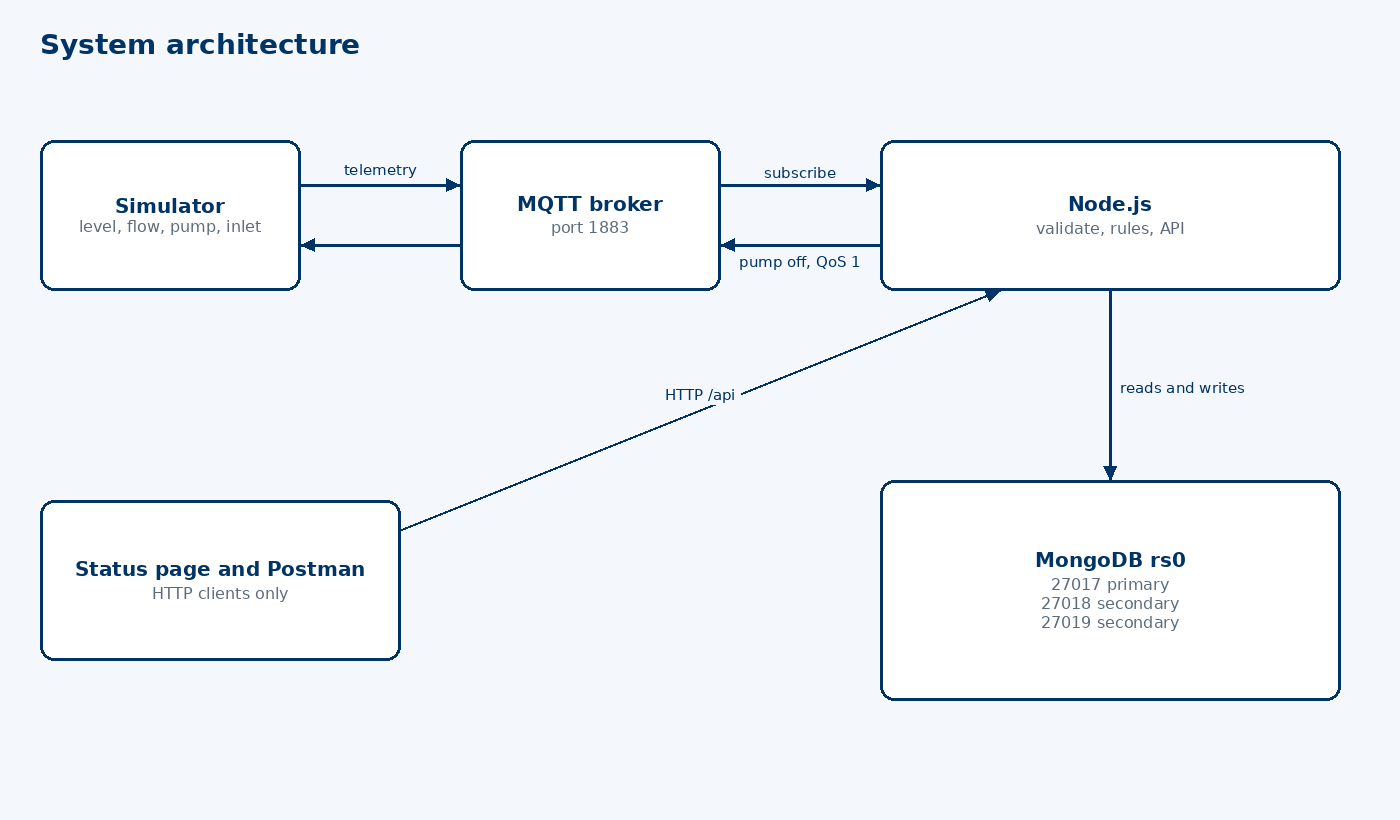
\includegraphics[width=0.9\textwidth]{../plan/img/system-architecture.png}
\caption{System architecture (placeholder): simulator $\rightarrow$ MQTT $\rightarrow$ Node.js ingest $\rightarrow$ MongoDB \texttt{rs0} $\rightarrow$ rule engine $\rightarrow$ MQTT command; REST API $\rightarrow$ status page and Telegram. Source file: \texttt{plan/img/system-architecture.png}.}
\label{fig:arch}
\end{figure}

% =====================================================================
\section{Types of NoSQL Databases and Selection of MongoDB}
% =====================================================================

NoSQL is not one technology but four broad families, each optimised for a different access pattern. A key--value store (for example Redis) maps opaque keys to opaque values with very low latency, which suits session caches and counters but offers little help when the application must query by device, subsystem, time range and severity. A wide-column store (for example Cassandra or HBase) distributes massive write workloads across many nodes with tunable consistency, which suits telecom-scale event ingestion but imposes a rigid column-family discipline that fits uniform counters better than variant sensor payloads. A graph store (for example Neo4j) traverses relationships between nodes, which suits fraud rings or social recommendations but adds machinery this household never uses: devices relate to exactly one subsystem, and no multi-hop traversal drives any rule. A document store (for example MongoDB or Couchbase) keeps each record as a self-describing JSON-like document, indexes any field, and varies the shape of one document without touching its neighbours.

Time-series extensions cut across these families. InfluxDB and TimescaleDB compress timestamped numeric streams efficiently, and MongoDB itself offers time-series collections. They were considered and set aside for two reasons. First, the dominant read in this system is not a range scan but a point lookup of current state: the rule engine and the status page need the latest document per device on every cycle, which \texttt{device\_latest} answers in one indexed query rather than a ``latest per group'' aggregation over history. Second, the interesting records --- rules, incidents, notifications --- are not numeric series at all but small operational documents with conditions, actions, escalation flags and delivery receipts. A pure series engine would force those back into a second store.

MongoDB was selected because the workload is document-shaped, query-shaped and availability-shaped in ways it answers directly. The polymorphic \texttt{reading} sub-document holds level, flow, pump, presence, lamp and climate payloads in one \texttt{telemetry} collection while per-type validation in the API keeps flexibility from becoming anarchy. Secondary indexes on \texttt{(subsystem\_id, device\_id, timestamp)} and on \texttt{device\_latest(subsystem\_id)} make both history charts and current-state joins cheap. Condition-list rules map naturally onto embedded arrays, and one open incident per rule is enforced with a partial unique index rather than application locking. The replica set supplies the availability mechanism the module assesses: three voting members, automatic election, majority write concern for the records that must survive a primary loss, and a lighter \texttt{w:1} for replaceable sensor history. Mongoose supplies schema validation, discriminated models per database, and \texttt{useDb} so one Node process serves three databases on the same set. Finally, the surrounding ecosystem --- the Node.js driver, Express, Mosquitto/Aedes MQTT clients, Compass and \texttt{mongosh} --- made every piece of required evidence (ingest logs, incident dumps, \texttt{rs.status()} transitions) collectable without extra infrastructure.

The alternatives were rejected on fit, not on quality. A key--value store cannot answer ``all open overflow incidents for this home, newest first'' without secondary indexing built by hand. A wide-column store would handle the write rate easily yet complicate the small-document operational workload and the ad-hoc coursework queries. A graph store would model the home--subsystem--device tree elegantly but never traverse it deeply enough to justify the engine. A dedicated series database would compress history well but split the system into two stores for no availability gain. MongoDB keeps one store, one query language and one replication story for the whole household.

\begin{figure}[h]
\centering
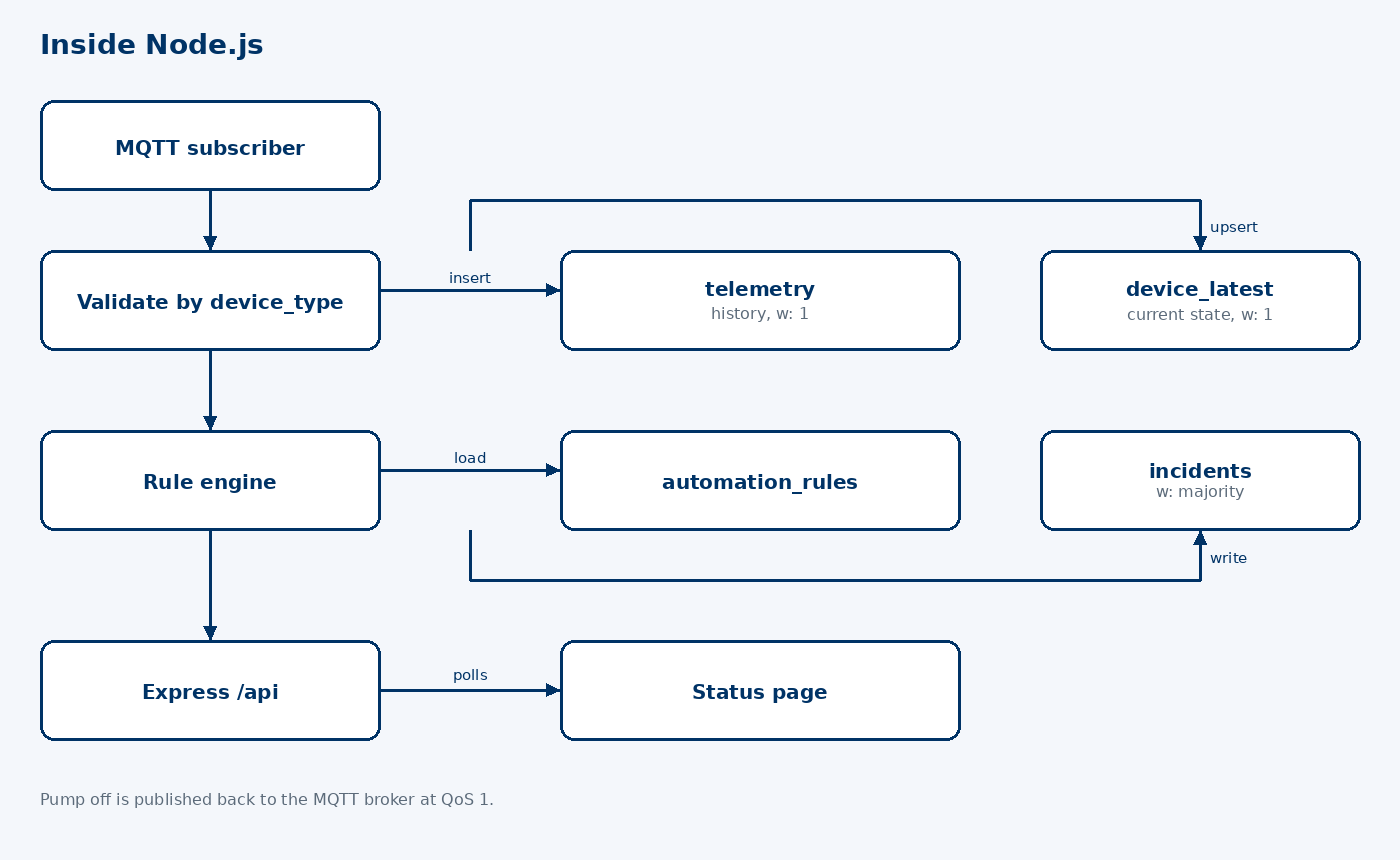
\includegraphics[width=0.75\textwidth]{../plan/img/node-flow.png}
\caption{Inside Node.js (placeholder): validation $\rightarrow$ \texttt{telemetry} insert (\texttt{w:1}) $\rightarrow$ \texttt{device\_latest} replace $\rightarrow$ subsystem rule evaluation $\rightarrow$ incident (\texttt{w:majority}) + MQTT command. Source: \texttt{plan/img/node-flow.png}.}
\label{fig:nodeflow}
\end{figure}

% =====================================================================
\section{Relational and NoSQL Database Comparison}
% =====================================================================

A relational design for this household is entirely possible, and its strengths should be stated fairly. Tanks, homes, devices, rules, incidents and notifications are well-bounded entities with stable keys; foreign keys would guarantee that no reading references a nonexistent device, and a single SQL statement could join tanks to devices to latest readings for a report. Multi-row ACID transactions would protect operations the business could not afford to half-complete, such as billing or stock decrements. The query language is standard, the tooling is mature, and any competent developer can read the schema on day one.

The friction appears exactly where the coursework lives: variant readings, evolving rules, and the ``current state'' read pattern. Three relational options exist for the reading, and each hurts. Option one is a single wide \texttt{reading} table with columns for every device type; most rows are then mostly null, every new sensor adds a column, and check constraints multiply. Option two is an entity--attribute--value table with one row per measured attribute; the schema never changes, but reconstructing one flow reading means pivoting several rows, and type safety moves into application code. Option three is a table per device type (\texttt{level\_reading}, \texttt{flow\_reading}, \texttt{pump\_reading}, \ldots); the schema is clean, but the status page must union or join N tables on every two-second poll, and adding the desk lamp means a DDL migration plus a new join branch. The document design avoids all three: one \texttt{telemetry} collection, one polymorphic \texttt{reading} field, validation per \texttt{device\_type} in \texttt{validateReading.js}, and indexes that serve both history and latest-state queries.

Rules widen the gap further. A water rule tests level, pump state, inlet presence and flow together; a desk rule tests presence, ambient light and lamp state; a climate rule tests temperature against the air-conditioner mode with a hysteresis band (cool above 28\textdegree C while off, stop at or below 26\textdegree C while cooling). In a relational schema each predicate shape wants its own columns or its own rule-type table, so every new automation revisits the DDL. Here each rule in \texttt{automation\_rules} is a condition list of \texttt{\{device\_type, field, operator, value\}} plus an \texttt{action} document; the desk and climate automations were added as data, seeding \texttt{rule\_study\_lamp}, \texttt{rule\_lamp\_off}, \texttt{rule\_cool\_on} and \texttt{rule\_cool\_off} without touching existing collections.

Consistency choices also differ by design rather than by default. A relational system typically applies the same transactional guarantee to every write. This system deliberately splits durability: high-frequency telemetry and \texttt{device\_latest} use \texttt{w:1} because a single lost sensor sample is replaced by the next one seconds later, while incidents use \texttt{w:majority} because an overflow cutoff or a confirmed fault must still be present after a primary failure. Reads use \texttt{primary} so the engine never decides from a lagging secondary. The failover run in \texttt{evidence/failover-election.log} and \texttt{evidence/rs-status-failover.json} shows why: after the 27018 primary was shut down, 27017 was elected within about three seconds (electionTime delta) and the cutoff incident written before the failure remained retrievable (see \texttt{evidence/failover-incident.json}).

Where the relational model still wins is integrity across entities: nothing in MongoDB stops a telemetry insert naming an unknown device except the application validator, whereas a foreign key would stop it at the store. That is accepted consciously. The validator, the per-topic subsystem check (message body must match the topic path), and the single-writer ingest path provide the practical guarantee, and the payoff is a store that absorbs new device types as documents rather than migrations. For an IoT household whose sensors change faster than its accounts, that trade favours documents.

% =====================================================================
\section{System Architecture}
% =====================================================================

The runtime has five stages. Simulators stand in for sensors and publish one MQTT message per device on topics of the form \texttt{ioThings/\{home\_id\}/\{subsystem\_id\}/\{device\_type\}/\{device\_id\}/telemetry}. The broker is the embedded Aedes instance on port 1883 when that port is free; if a system Mosquitto already holds it, the API attaches to that broker instead, so simulator commands never change. The Node.js ingest path (\texttt{ingest.js}, \texttt{mqtt.js}) parses the topic, rejects bodies whose subsystem disagrees with the path, validates the payload by \texttt{device\_type}, inserts into \texttt{telemetry} at \texttt{w:1}, replaces the matching \texttt{device\_latest} document, and then runs the rule engine for that subsystem only (water evaluator versus room evaluator). Commands return along \texttt{\ldots/command} at QoS~1: \texttt{motor\_state} off/on for the pump, \texttt{study}/off for the lamp, \texttt{cool}/off for the climate unit. The status page (\texttt{backend/src/public/index.html} served by Express at \texttt{http://localhost:3000}) polls the API every two seconds and never touches MongoDB or MQTT directly; manual Off/On buttons travel through \texttt{POST /motors/:deviceId/override}, which records a \texttt{manual\_override} incident, stores a notification, and publishes the command. Figure~\ref{fig:arch} summarises the loop; Figure~\ref{fig:overflow} traces the overflow path.

Persistence sits behind the API on the replica-set URI with \texttt{readPreference=primary}. One Mongoose connection fans out through \texttt{useDb} to the three databases, so the subsystem type found by \texttt{resolveSubsystem} selects the correct models for every read and write. Because history (\texttt{telemetry}) and current state (\texttt{device\_latest}) share the same key shape, the join the page needs on every poll is a small indexed query by \texttt{subsystem\_id} rather than an aggregation over time series. Notifications close the loop to the person: each incident writes exactly one notification document, and the Telegram sender delivers the same text only when both the bot token and the chat identifier are configured, otherwise marking the receipt as on-page delivery.

\begin{figure}[h]
\centering
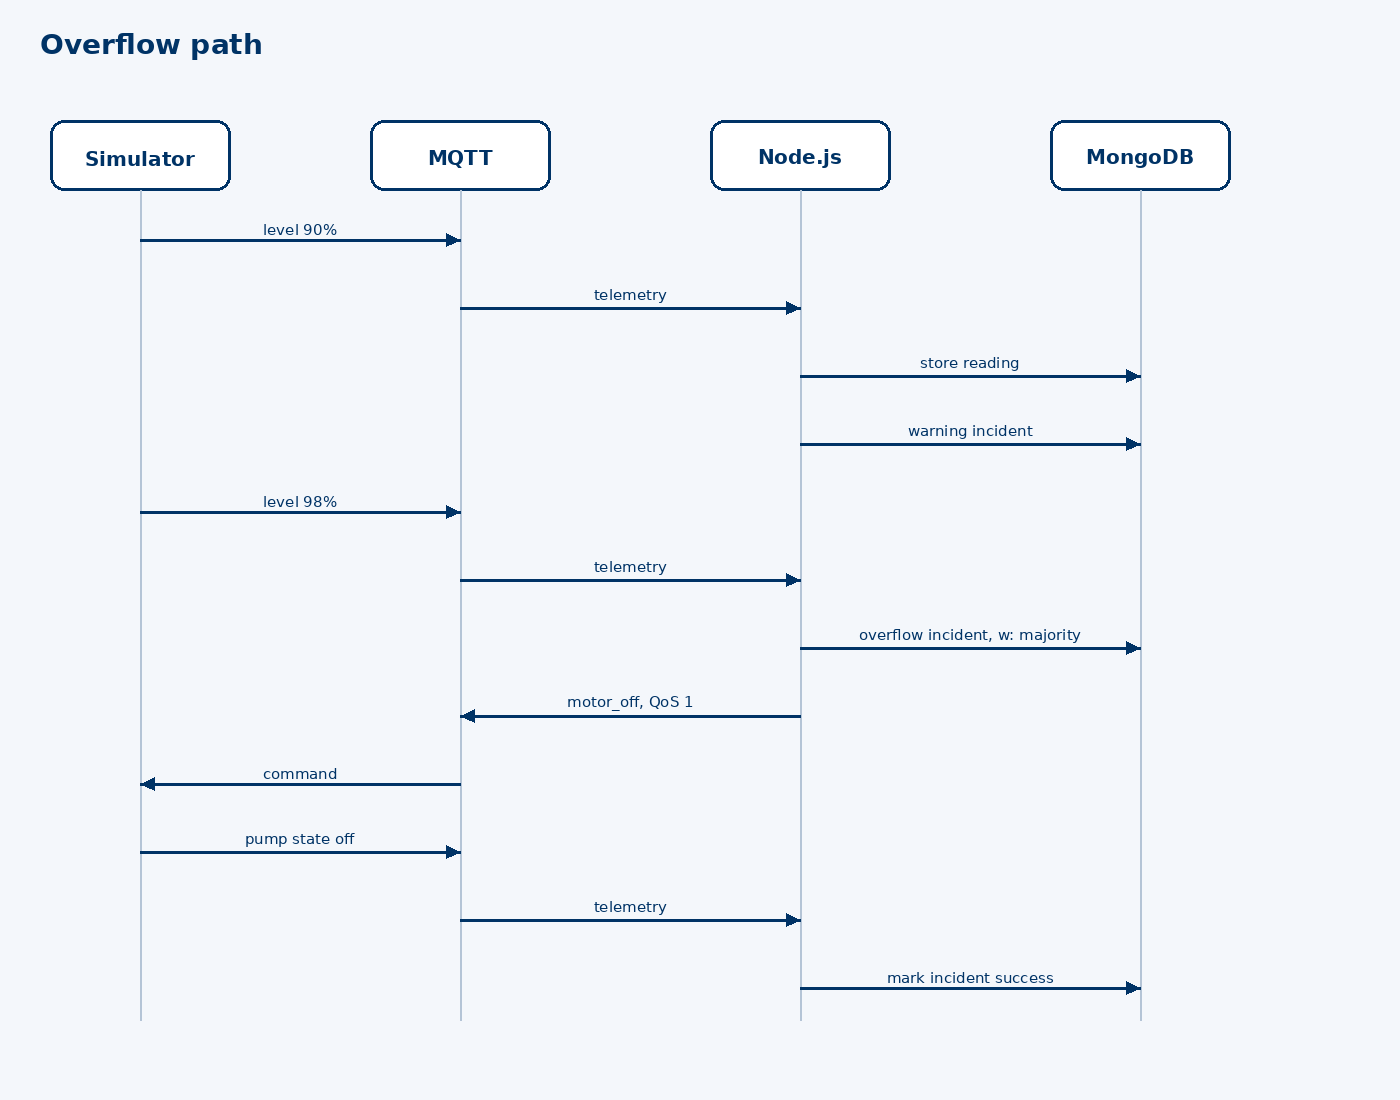
\includegraphics[width=0.9\textwidth]{../plan/img/overflow-sequence.png}
\caption{Overflow path (placeholder): 90\% warning $\rightarrow$ 98\% cutoff command $\rightarrow$ incident (\texttt{w:majority}) + Telegram $\rightarrow$ simulator applies off. Source: \texttt{plan/img/overflow-sequence.png}.}
\label{fig:overflow}
\end{figure}

% =====================================================================
\section{NoSQL Database Design}
% =====================================================================

\subsection{Dataset and Device Fleet}

Three databases share replica set \texttt{rs0}: \texttt{smart\_water}, \texttt{smart\_focus} and \texttt{smart\_climate}, selected per subsystem through \texttt{useDb}. Only \texttt{smart\_water} holds a \texttt{tanks} collection (seeded \texttt{tank\_roof\_01}, capacity 1000~L, thresholds 90/98/15). Every database holds \texttt{subsystems}, \texttt{devices}, \texttt{telemetry}, \texttt{device\_latest}, \texttt{automation\_rules}, \texttt{incidents} and \texttt{notifications}; every document carries \texttt{subsystem\_id} so a water reading can never land in the climate collections and home-wide lists merge the three stores sorted by time. The water fleet is four devices: \texttt{tank\_level\_roof\_01} (\texttt{level\_pct}, \texttt{level\_cm}), \texttt{water\_flow\_roof\_01} (\texttt{flow\_rate\_lpm}, \texttt{cumulative\_litres}, \texttt{direction}), \texttt{motor\_roof\_01} (\texttt{state}, \texttt{runtime\_seconds}), and \texttt{source\_roof\_01} (\texttt{water\_present}). The desk adds presence, ambient-light and lamp devices; climate adds temperature and air-conditioner devices.

\subsection{Document Structure}

A telemetry document \texttt{\{home\_id, subsystem\_id, tank\_id?, device\_id, device\_type, reading, timestamp\}} keeps routable fields at top level for indexing and nests only the variant payload inside \texttt{reading}. \texttt{device\_latest} mirrors the same shape with one document per device, updated by replacement. A rule document holds \texttt{rule\_id}, \texttt{subsystem\_id}, an \texttt{enabled} flag, a \texttt{conditions} array and an \texttt{action}; multi-sensor water rules additionally require the referenced readings to be mutually current, so a stale flow value from before a pump transition cannot fire them, and at most one open incident per \texttt{rule\_id} is kept (an old open fault otherwise masks a new overflow until acknowledged). An incident records \texttt{severity}, \texttt{triggered\_by} snapshots, \texttt{action\_taken} with status (\texttt{success}/\texttt{pending}/\texttt{cleared}), and, for cutoffs, \texttt{litres\_saved} $=$ flow $\times$ 20 with the assumed 20 unattended minutes stored alongside so the estimate is auditable. Derived figures --- litres in tank (capacity $\times$ level/100), litres and minutes to the 98\% cutoff (only while pumping with positive flow) --- are computed on read in \texttt{tankService.js} and never stored, so they cannot drift from their source sensors. Key indexes cover telemetry time queries, latest-state lookups, and open-incident guards.

\begin{center}
\small
\begin{tabularx}{\textwidth}{@{}lXX@{}}
\toprule
Severity & Fires when & Action \\
\midrule
\texttt{warning} & level $\ge$ 90\% and pump on & incident only (person may press Off $\approx$ 95\%) \\
\texttt{overflow\_prevented} & level $\ge$ 98\% and pump on & pump off + incident; litres\_saved $=$ flow $\times$ 20 \\
\texttt{dry\_run} & pump on and inlet absent & pump off + incident \\
\texttt{pump\_failure} & pump on, water present, $\approx$0 flow, level flat & incident only \\
\texttt{abnormal\_flow} & pump off but flow $>$ 0 & incident only \\
\texttt{low\_water} & level $\le$ 15\% and pump off & incident only \\
\texttt{confirmed\_fault} & off sent, pump still on after 30~s & escalate open incident \\
\texttt{manual\_override} & Off/On pressed on page & MQTT command + incident \\
\bottomrule
\end{tabularx}
\end{center}

The inlet boolean is the diagnostic pivot: dry-run and pump-failure both show a pump that is on with a non-rising level, but only dry-run shows \texttt{water\_present} false.

% =====================================================================
\section{Implementation}
% =====================================================================

\subsection{End-to-End Runtime Flow}

Each cycle is identical across subsystems. The simulator publishes a per-device reading; ingest validates, writes history, refreshes \texttt{device\_latest}, and evaluates only the enabled rules of that subsystem against current values. The water evaluator checks the warning, cutoff, dry-run, pump-failure, abnormal-flow and low-water rules in severity order; the room evaluator checks the lamp pair (present $\rightarrow$ \texttt{lamp\_study} at 6500~K/100\%; absent $\rightarrow$ \texttt{lamp\_off}, skipped when already in target state) and the climate pair with its 26/28\textdegree C hysteresis so the unit does not chatter at one threshold. Firing opens an incident at \texttt{w:majority}, stores a notification, optionally publishes a QoS~1 command, and --- when Telegram credentials are configured --- sends the same text to the configured chat. The simulator then applies the command and publishes the resulting device state, which is what the next page poll displays. The 30-second \texttt{confirmed\_fault} timer watches every off command: if the pump still reports on, the open cutoff incident is marked escalated rather than opening a duplicate.

Concretely the water cycle is: level, flow, pump and inlet messages arrive within the same second; \texttt{ingest.js} writes four telemetry documents and replaces four latest-state documents; \texttt{rules/engine.js} loads the enabled rules for \texttt{tank\_roof\_01} from \texttt{automation\_rules} and tests their condition lists in \texttt{rules/conditions.js}; a firing rule calls \texttt{rules/actions.js}, which publishes the MQTT command and persists the incident plus notification through \texttt{services/}; the simulator receives the command, updates its internal pump flag, and its next telemetry batch reflects the new state, closing the feedback loop. Desk and climate cycles reuse the same files with different evaluators and command vocabularies, which is why one developer can reason about all three automations from a single code path.

\subsection{Software Installation and Commands}

Prerequisites are Node.js 18+, a local \texttt{mongod} triple on 27017--27019 initialised once as \texttt{rs0} (never re-initiate), and optionally Mosquitto. Setup is \texttt{npm install}, \texttt{scripts/replica-up.sh}, \texttt{npm run seed} (three subsystems, devices, rules), \texttt{npm run dev} (API + Aedes on 1883 if free). Simulation is \texttt{npm run simulate -- <normal|overflow|dry-run|pump-failure|abnormal-flow|fault|study|cool>}; only one tank scenario runs at a time while \texttt{study} and \texttt{cool} may overlap the tank on disjoint topics. \texttt{cool} loops between heating (+0.6\textdegree C/s while off) and cooling ($-$0.5\textdegree C/s to a 24\textdegree C floor) and must be stopped after the recorded cycle. Telegram needs \texttt{TELEGRAM\_BOT\_TOKEN} and \texttt{TELEGRAM\_CHAT\_ID} in \texttt{.env} before the API starts; without them notifications are still stored and shown on the page as on-page only.

The seed writes fixed identifiers so evidence is reproducible: home \texttt{home\_001}, tank \texttt{tank\_roof\_01} at 1000~litres, pump \texttt{motor\_roof\_01}, and the full rule set (\texttt{rule\_warning\_roof}, \texttt{rule\_overflow\_roof}, \texttt{rule\_dry\_run\_roof}, \texttt{rule\_pump\_failure\_roof}, \texttt{rule\_abnormal\_flow\_roof}, \texttt{rule\_low\_water\_roof}, plus the desk and climate rules). The \texttt{normal} scenario fills while pumping and drains after switch-off, exercising the falling-level path that clears the low-water incident; \texttt{overflow} climbs 80\% to 98\% and holds; \texttt{dry-run} publishes inlet absent with the pump on; \texttt{pump-failure} publishes inlet present with near-zero flow and a flat level; \texttt{abnormal-flow} publishes flow while the pump is off; \texttt{fault} acknowledges no command so the escalation timer can be observed.

\subsection{Implementation Evidence Screenshots}

To be captured for the appendix: API process log (\texttt{evidence/api-process.log}, health in \texttt{evidence/api-health.json}); overflow simulator trace (\texttt{evidence/overflow-simulator.log}) showing the 80\% $\rightarrow$ 98\% climb and the cutoff incident with \texttt{litres\_saved} 300 (15~L/min $\times$ 20); fault trace (\texttt{evidence/fault-simulator.log}, \texttt{evidence/confirmed-fault-incident.json}) showing the ignored off command and escalation; notification dumps (\texttt{evidence/fault-notifications.json}); replica states before, during and after failover (\texttt{evidence/rs-status-before.json}, \texttt{evidence/rs-status-failover.json}, \texttt{evidence/rs-status-rejoined.json}, \texttt{evidence/failover-election.log}).

\begin{figure}[h]
\centering
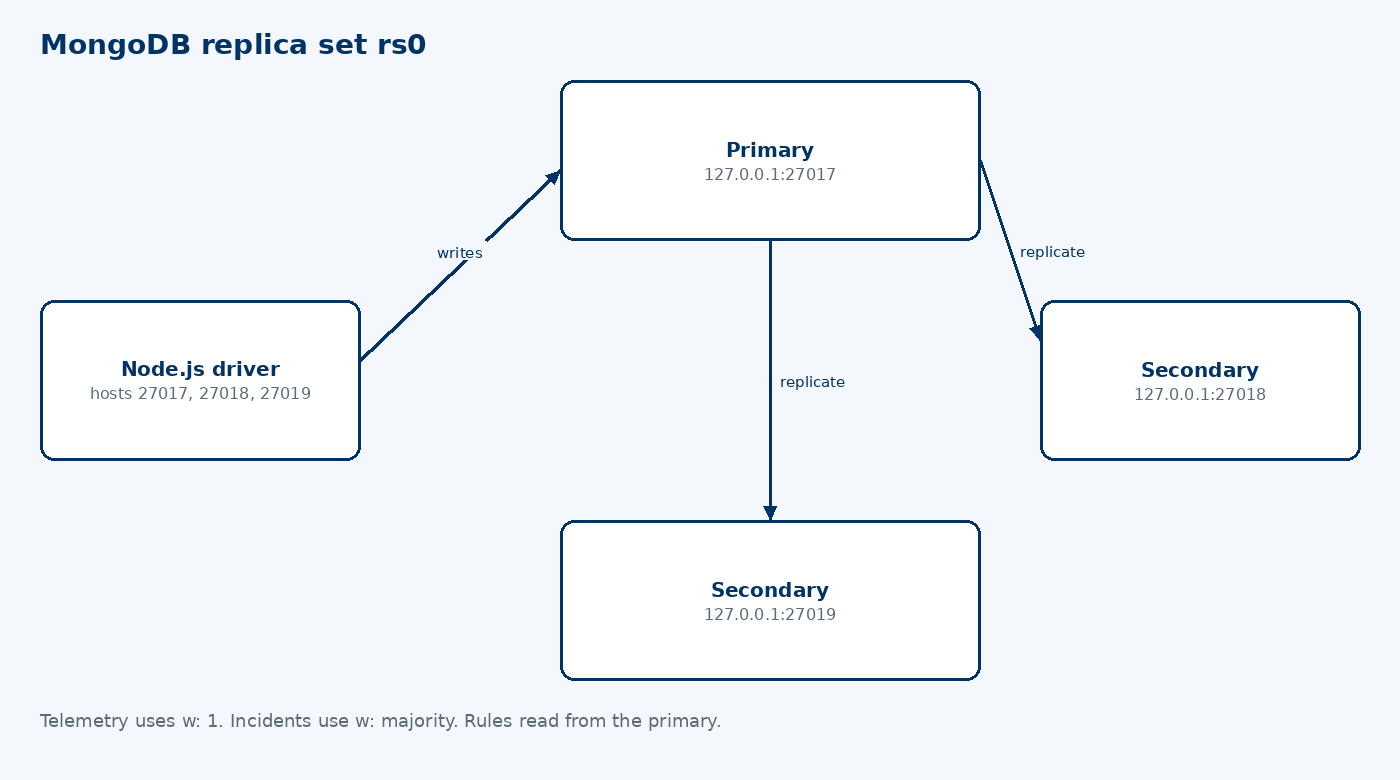
\includegraphics[width=0.7\textwidth]{../plan/img/replica-set.png}
\caption{Replica set \texttt{rs0} (placeholder): primary 27018 $\rightarrow$ failover to 27017 $\rightarrow$ rejoin as secondary. Source: \texttt{plan/img/replica-set.png}.}
\label{fig:rs}
\end{figure}

% =====================================================================
\section{Data Management}
% =====================================================================

Data quality is enforced at the boundary, not wished for afterwards. Every ingest passes three gates: the topic parses to the four-part path, the body names the same \texttt{subsystem\_id}, and \texttt{validateReading.js} accepts the payload shape for its \texttt{device\_type} (ranges for level and flow, enum states for pump, lamp and climate). Failures are rejected before any write, so malformed simulator output cannot poison history or trigger rules. Freshness is enforced inside the engine: multi-sensor rules compare the timestamps of the readings they consume and refuse to fire on a mixture of new pump state with old flow. Lifecycle policy keeps history append-only while \texttt{device\_latest} is a bounded working set of one document per device, so read cost is independent of retention. Derived values (litres, minutes to cutoff) are recomputed on read. Notifications are write-once records with a delivery receipt (\texttt{channel}, \texttt{delivered}); Telegram is a best-effort sender over a durable store, meaning a missing token or rejected chat never loses the alert --- it only changes the receipt to on-page. Finally, incident closure is explicit: overflow incidents resolve when the command succeeds, low-water clears when the level recovers or the pump starts, and faults stay open until acknowledged through the API, which is why at most one open incident per rule is the correct guard.

% =====================================================================
\section{REST API, Swagger and Dashboard}
% =====================================================================

\subsection{API Design}

The Express API at \texttt{http://localhost:3000/api} exposes \texttt{GET /health} (process, broker, replica members), full CRUD for \texttt{/tanks}, \texttt{/devices} and \texttt{/rules}, \texttt{POST /telemetry} plus range queries, \texttt{GET /incidents} with \texttt{/incidents/stats} and per-incident \texttt{PATCH} acknowledgement, \texttt{POST /motors/:deviceId/override} for manual pump commands, notification listing, and replica-status reporting. Semantics are uniform: collection GETs paginate and filter by subsystem, POSTs validate before writing, and incident writes carry \texttt{w:majority} while telemetry writes carry \texttt{w:1}. Manual overrides are first-class incidents rather than silent publishes, so the audit trail shows who (page) commanded what and when.

\subsection{Dashboard Design}

The single-file status page opens as a room launcher (Water, Light, Climate, Alerts) and polls every two seconds. The water view shows level, litres, flow, pump and inlet state, minutes-to-cutoff while pumping, history chart, running totals (incidents, litres saved), and acknowledge buttons; the desk and climate views show presence/lamp and temperature/AC state respectively. Because the page reads only the API, every number on screen is proof that MQTT $\rightarrow$ MongoDB $\rightarrow$ REST is working rather than a hard-coded mock.

API and dashboard evidence to attach: health JSON (\texttt{evidence/api-health.json}), incident summary (\texttt{evidence/incidents-summary.log}), notification summary (\texttt{evidence/fault-notifications-summary.log}), and page screenshots for the warning banner ($\approx$92\%), the cutoff state (98\%, pump off, 300~L saved), the confirmed-fault escalation, and the desk/climate views. Swagger-style request/response captures for \texttt{/health}, \texttt{/devices}, \texttt{/telemetry}, \texttt{/incidents} and \texttt{/incidents/stats} belong alongside them; where formal Swagger UI is unavailable, \texttt{mongosh} dumps and browser captures serve the same evidential role.

% =====================================================================
\section{Testing}
% =====================================================================

Testing is scenario-based against the live stack. Each simulator case is a test: \texttt{normal} must fill then drain with no cutoff incident; \texttt{overflow} must raise a 90\% warning then a 98\% cutoff with pump off and 300~L saved; \texttt{dry-run} and \texttt{pump-failure} must open their respective incidents with the inlet boolean as the only distinguishing snapshot; \texttt{abnormal-flow} must fire while the pump is off; \texttt{fault} must escalate to \texttt{confirmed\_fault} after 30~s; \texttt{study} must drive the lamp to 6500~K/100\% then off; \texttt{cool} must start cooling above 28\textdegree C and stop at 26\textdegree C. Pass criteria are checked in \texttt{mongosh} (incident documents, \texttt{triggered\_by} snapshots, action statuses) and on the page (banners, totals, acknowledgement). Recorded runs already show the overflow warning/cutoff pair, the dry-run/pump-failure/abnormal-flow incidents, and the fault escalation with two Telegram-marked notifications.

\begin{center}
\small
\begin{tabularx}{\textwidth}{@{}lll@{}}
\toprule
Case & Must open & Must show \\
\midrule
\texttt{normal} & low-water only at $\le$15\% & level falls after pump stops \\
\texttt{overflow} & warning + cutoff & pump off, 300~L saved \\
\texttt{dry-run} / \texttt{pump-failure} & respective incident & inlet snapshot differs \\
\texttt{abnormal-flow} & abnormal-flow & no pump command \\
\texttt{fault} & escalation after 30~s & open incident marked escalated \\
\texttt{study} / \texttt{cool} & lamp / climate incidents & actuator follows state \\
\bottomrule
\end{tabularx}
\end{center}

Full automation under \texttt{npm test} and negative tests (malformed payloads, stale-timestamp mixes, double-acknowledgement) remain future work; the evidence logs above are the current proof set. Regression discipline is procedural for now: re-seed, run each tank scenario alone, confirm the incident set in \texttt{mongosh} matches the table, and only then record screenshots, because a stray second simulator on the same topics would interleave readings and invalidate the run.

% =====================================================================
\section{Distribution and Clustering}
% =====================================================================

Distribution in this project means a replica set, and the coursework asks that its behaviour be demonstrated rather than asserted. A replica set keeps identical data on several \texttt{mongod} processes, elects one primary to take writes, replicates the operation log to secondaries, and elects a new primary automatically when the old one disappears, provided a majority of voting members remains. Three members on 27017--27019 is the smallest configuration that tolerates one failure while still reaching a majority of two; a single-node ``replica set'' would prove configuration syntax but nothing about availability, so three local processes are used.

Configuration is straightforward. Each member runs with \texttt{--replSet rs0} and a distinct port and data directory; the set is initiated once naming all three members; the application connects with \texttt{mongodb://127.0.0.1:27017,127.0.0.1:27018,127.0.0.1:27019/smart\_water?replicaSet=rs0} and \texttt{readPreference=primary}. All application reads specify the primary so rules never act on replicated-lag state. Telemetry and \texttt{device\_latest} write at \texttt{w:1}: the write returns once the primary has it, which keeps per-second sensor traffic fast at the cost that a primary crash in the same instant could lose that one sample --- acceptable because the next sample arrives seconds later. Incidents write at \texttt{w:majority}: the write returns only once two of three members hold it, so a cutoff or fault record acknowledged to the engine survives the loss of any single node. That split is the central availability argument of the report: cheap speed where data is replaceable, majority durability where data is the safety record.

The health endpoint exposes the set truthfully. When connected to \texttt{rs0} it returns the set name, each member's address, state string and health flag; when pointed at a standalone server it says so instead of inventing members. \texttt{scripts/replica-status.sh} and the \texttt{rs.status()} captures provide the same information out of band.

Failover was exercised, not assumed. With the system mid-overflow, the primary on 27018 was shut down at 17:21:39Z; the next poll showed 27017 as primary and 27018 unreachable with 27019 secondary, and electionTime comparison places the election about three seconds after the shutdown command (the longer wall-clock span in the log includes the shutdown handshake). The cutoff incident written before the failure (\texttt{inc\_1790788742795}, \texttt{flow\_rate\_lpm} 15, \texttt{litres\_saved} 300) remained readable through the new primary, and the fault notification pair for the same window was intact; the stopped member was restarted and rejoined as a secondary, confirmed in \texttt{rs-status-rejoined.json} and \texttt{replica-status-final.log}. During the window without a primary, sensor writes pause rather than silently diverging, which is correct primary-preferring behaviour for a safety system: no split-brain cutoff, no lost majority incident.

Backup, recovery and scale complete the picture. \texttt{mongodump} against the primary (or a secondary with \texttt{--oplog} for point-in-time capture) backs all three databases; restore replays into a fresh set, and the seed script rebuilds subsystem/device/rule fixtures deterministically if a logical rebuild is preferred. Sharding is not deployed --- three replicas of a household workload do not need it --- but the shard-key choice is recorded for the high-volume collection: \texttt{telemetry} would shard on \texttt{\{subsystem\_id: 1, timestamp: 1\}} (or \texttt{\{device\_id: 1, timestamp: 1\}}), keeping each subsystem's history together while distributing time ranges, and \texttt{device\_latest} would stay unsharded as a small lookup collection. Production would separate the members onto different hosts or availability zones; co-location here is a coursework constraint, and the election logic demonstrated is identical either way.

\begin{lstlisting}[caption={Replica URI used by server and evidence (placeholder for screenshot).},label={lst:uri}]
MONGO_URI=mongodb://127.0.0.1:27017,127.0.0.1:27018,127.0.0.1:27019/smart_water?replicaSet=rs0
\end{lstlisting}

% =====================================================================
\section{Security, Operations and Future Work}
% =====================================================================

This is a prototype, and its trust boundaries are stated openly. MongoDB runs without authentication, the broker accepts anonymous local clients, the API exposes no login, and Telegram credentials sit in \texttt{.env}. That is acceptable on an isolated coursework machine and unacceptable anywhere else. Production would enable MongoDB keyfile/SCRAM authentication with role-separated users, MQTT username/password plus TLS, API authentication and rate limiting, secrets management instead of flat files, and validation already present extended with JSON-schema collection validators. Operationally the system is already well-behaved: replica scripts for up/down/status, a health endpoint that reports broker and set state, append-only history with a bounded latest-state set, and explicit acknowledgement so stale open faults cannot mask new overflows silently. Future work is a phone client on the existing API, automated tests with negative cases, formal Swagger UI, per-home multi-tenancy, and sharded telemetry if device counts grow by orders of magnitude.

MongoDB and distribution evidence to attach: Compass views of \texttt{telemetry}, \texttt{device\_latest}, \texttt{automation\_rules}, \texttt{incidents} and \texttt{notifications}; index listings; the three \texttt{rs.status()} captures; and the election/rejoin logs. Items still requiring fresh screenshots are marked [CAPTURE] in the appendix checklist below.

% =====================================================================
\section{Conclusion}
% =====================================================================

One household, three document databases, one replica set. MQTT brings each reading in and carries each command out; the rule engine turns current state into incidents with majority durability; the page and Telegram turn incidents into human action. The roof tank warns at 90\%, stops itself at 98\% with an auditable litres-saved estimate, tells dry-run from pump-failure by the inlet sensor, and escalates ignored commands after 30~seconds. Desk and climate reuse the same path with their own rules. The evaluation shows the document model fits variant readings and condition-list rules better than fixed tables, the write-concern split protects safety records without slowing sensor traffic, and the failover run proves the cutoff survives a primary loss. No new sensor requires a migration, no safety record depends on a single node, and no alert depends on a single delivery channel. The remaining work is evidence capture, above all the dashboard, Compass and Swagger screenshots, rather than any change to that loop.

\begin{thebibliography}{9}
\bibitem{banks2014} Banks, A. and Gupta, R. (eds.) (2014) \textit{MQTT Version 3.1.1}. OASIS Standard. Available at: \url{https://docs.oasis-open.org/mqtt/mqtt/v3.1.1/os/mqtt-v3.1.1-os.html} [Accessed 30 September 2026].
\bibitem{mongo-repl} MongoDB, Inc. (2026a) \textit{Replication and replica sets}. MongoDB Manual. Available at: \url{https://www.mongodb.com/docs/manual/replication/} [Accessed 30 September 2026].
\bibitem{mongo-wc} MongoDB, Inc. (2026b) \textit{Write concern}. MongoDB Manual. Available at: \url{https://www.mongodb.com/docs/manual/reference/write-concern/} [Accessed 30 September 2026].
\bibitem{mongo-index} MongoDB, Inc. (2026c) \textit{Indexes}. MongoDB Manual. Available at: \url{https://www.mongodb.com/docs/manual/indexes/} [Accessed 30 September 2026].
\bibitem{mongo-model} MongoDB, Inc. (2026d) \textit{Data modeling: flexible schema}. MongoDB Manual. Available at: \url{https://www.mongodb.com/docs/manual/core/data-modeling-introduction/} [Accessed 30 September 2026].
\bibitem{express} OpenJS Foundation (2026) \textit{Express --- Node.js web application framework}. Available at: \url{https://expressjs.com/} [Accessed 30 September 2026].
\bibitem{mosquitto} Eclipse Foundation (2026) \textit{Eclipse Mosquitto documentation}. Available at: \url{https://mosquitto.org/documentation/} [Accessed 30 September 2026].
\bibitem{strauch} Strauch, C. (2011) \textit{NoSQL databases}. Stuttgart: Stuttgart Media University. Available at: \url{https://www.christof-strauch.de/nosqldbs.pdf} [Accessed 30 September 2026].
\bibitem{sadalage} Sadalage, P. and Fowler, M. (2012) \textit{NoSQL distilled: a brief guide to the emerging world of polyglot persistence}. Boston: Addison-Wesley.
\end{thebibliography}

\appendix
\section*{Appendix A --- Evidence checklist}
\begin{center}
\small
\begin{tabularx}{\textwidth}{@{}lXl@{}}
\toprule
Figure & File & State \\
\midrule
Architecture diagram & \texttt{plan/img/system-architecture.png} & present \\
Node ingest flow & \texttt{plan/img/node-flow.png} & present \\
Replica-set diagram & \texttt{plan/img/replica-set.png} & present \\
Overflow sequence & \texttt{plan/img/overflow-sequence.png} & present \\
API health & \texttt{evidence/api-health.json} & present \\
Overflow trace & \texttt{evidence/overflow-simulator.log} & present \\
Fault trace + escalation & \texttt{evidence/fault-simulator.log}, \texttt{evidence/confirmed-fault-incident.json} & present \\
Notifications | \texttt{evidence/fault-notifications.json} & present \\
Replica states + election & \texttt{evidence/rs-status-before.json}, \texttt{evidence/rs-status-failover.json}, \texttt{evidence/rs-status-rejoined.json}, \texttt{evidence/failover-election.log} & present \\
Dashboard screenshots (warning/cutoff/fault/desk/climate) & \texttt{evidence/} & [CAPTURE] \\
Compass collection + index screenshots & \texttt{evidence/} & [CAPTURE] \\
Swagger/response captures & \texttt{evidence/} & [CAPTURE] \\
\bottomrule
\end{tabularx}
\end{center}

\end{document}
